% Figure s01f03_threechannels (Session 1): one Hamiltonian and three ordered states.
% The image is rendered by figures/blender/s01f03_threechannels.py; the coordinates of the labels come from
% figures/blender/out/s01f03_threechannels_anchors.tex. Build with figures/blender/build_figure.sh s01f03_threechannels.
\documentclass[11pt,tikz,border=0pt]{standalone}
\usepackage[T1]{fontenc}
\usepackage{amsmath,amssymb,graphicx}
\usepackage{xcolor}
\usetikzlibrary{arrows.meta}
% The three label colors of the figures, with the same values as in src/figures_preamble.tex.
\definecolor{aqmaccent}{RGB}{31,78,121}
\definecolor{aqmbroken}{RGB}{168,42,34}
\definecolor{aqmmuted}{RGB}{125,125,125}

\newlength{\figw}\setlength{\figw}{15.6cm}   % the text width of the notes (A4, 2.7 cm margins)

\begin{document}
\begin{tikzpicture}[lbl/.style={font=\small, inner sep=1.5pt},
    flow/.style={line width=0.9pt, -{Stealth[length=5pt,width=4pt]}}]
  \node[anchor=south west, inner sep=0pt] at (0,0)
    {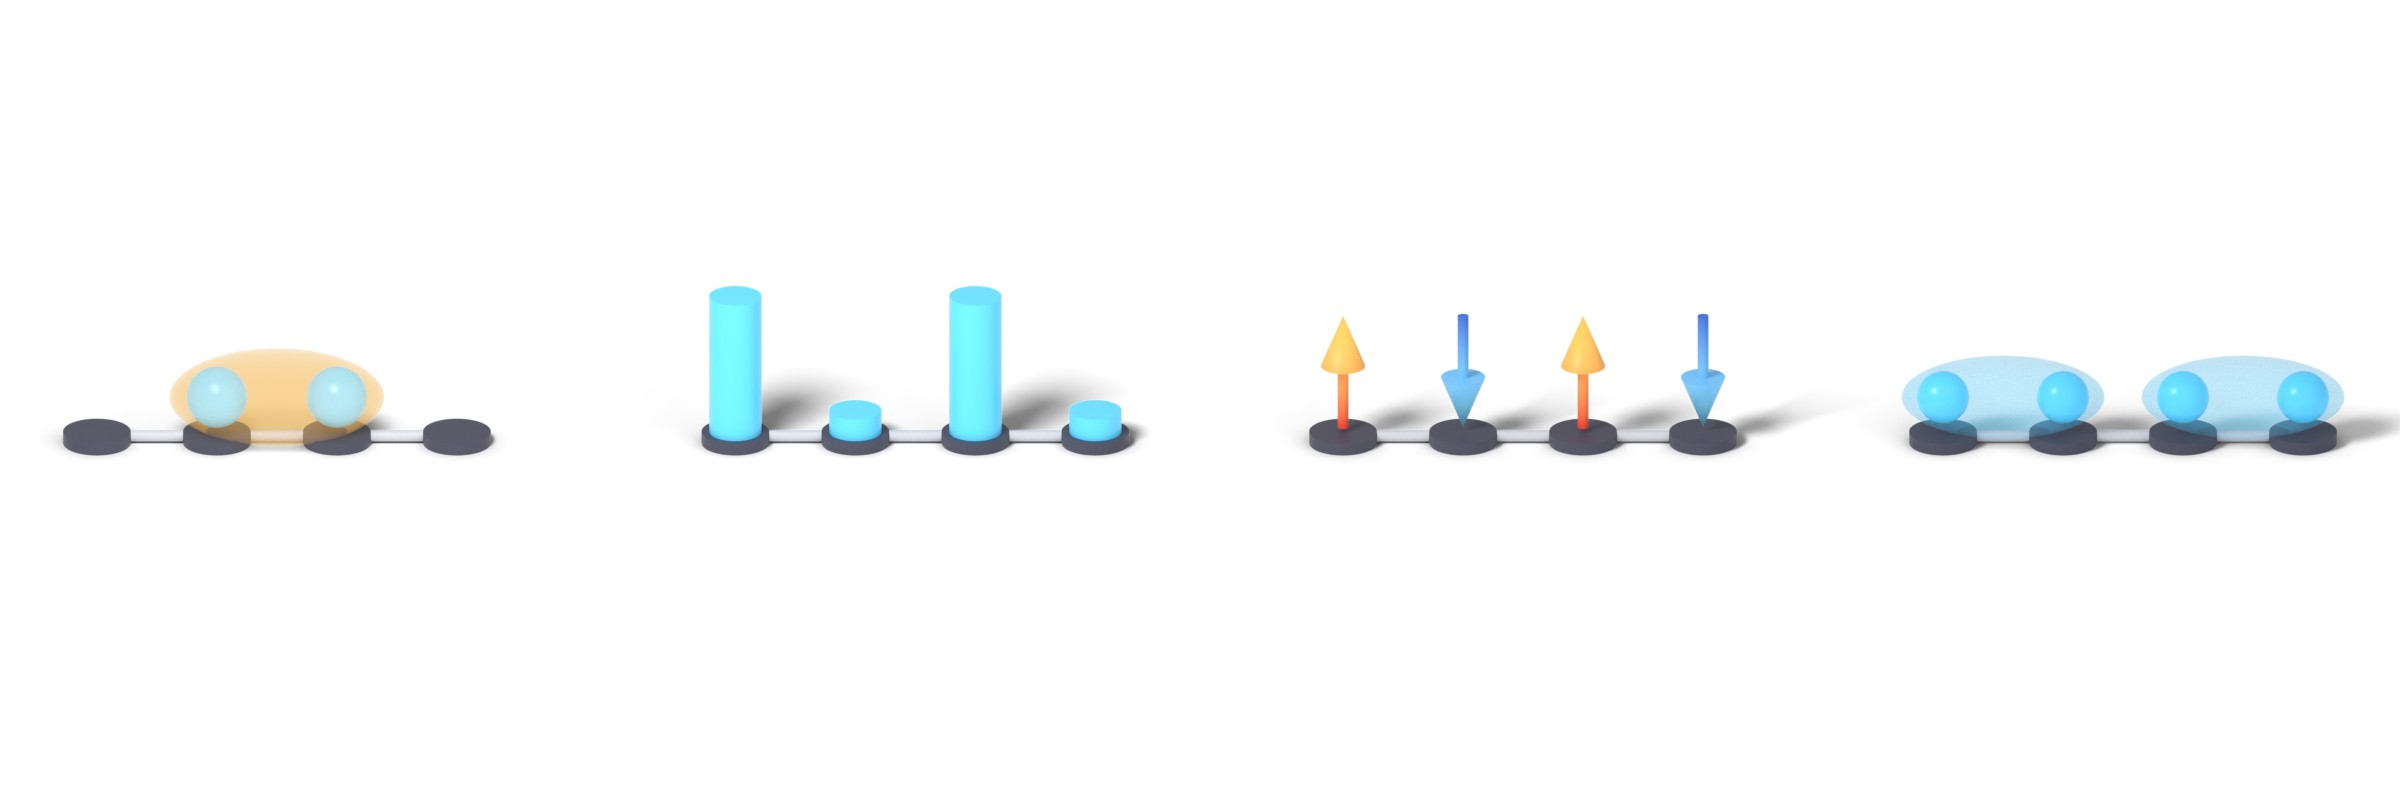
\includegraphics[width=\figw]{../blender/out/s01f03_threechannels.jpg}};
  %% written by figlib.py; x and y in units of the image width
\coordinate (H) at (0.1154\figw,0.2112\figw);
\coordinate (Hb) at (0.1154\figw,0.1392\figw);
\coordinate (out) at (0.2276\figw,0.1696\figw);
\coordinate (in0) at (0.2853\figw,0.1696\figw);
\coordinate (top0) at (0.3814\figw,0.2172\figw);
\coordinate (bot0) at (0.3814\figw,0.1392\figw);
\coordinate (in1) at (0.5385\figw,0.1696\figw);
\coordinate (top1) at (0.6346\figw,0.2172\figw);
\coordinate (bot1) at (0.6346\figw,0.1392\figw);
\coordinate (in2) at (0.7885\figw,0.1696\figw);
\coordinate (top2) at (0.8846\figw,0.2172\figw);
\coordinate (bot2) at (0.8846\figw,0.1392\figw);

  \node[lbl, anchor=south, text=aqmaccent] at (H) {$V_{ijkl}$};
  \node[lbl, anchor=north, align=center] at (Hb)
    {$H=\sum_{ij}t_{ij}\,c_i^\dagger c_j$\\[1pt]$+\sum_{ijkl}V_{ijkl}\,c_i^\dagger c_j^\dagger c_k c_l$\\[1pt]
     \textcolor{aqmmuted}{eq.~(1.5)}};
  \draw[flow, aqmaccent] (out) -- node[lbl, above, align=center] {mean\\field} (in0);
  \node[lbl, anchor=south, align=center] at (top0) {$\langle c_n^\dagger c_n\rangle$};
  \node[lbl, anchor=south, align=center] at (top1)
    {$\langle c_{n\uparrow}^\dagger c_{n\uparrow}\rangle-\langle c_{n\downarrow}^\dagger c_{n\downarrow}\rangle$};
  \node[lbl, anchor=south, align=center] at (top2) {$\langle c_i c_j\rangle$};
  \node[lbl, anchor=north, align=center] at (bot0)
    {charge density wave\\breaks \textbf{translational}\\\textcolor{aqmmuted}{eq.~(1.6)}\\\textcolor{aqmmuted}{not revisited}};
  \node[lbl, anchor=north, align=center] at (bot1)
    {magnet\\breaks \textbf{time-reversal}\\\textcolor{aqmmuted}{eqs.~(1.7) and (1.8)}\\\textcolor{aqmmuted}{again in session 6}};
  \node[lbl, anchor=north, align=center] at (bot2)
    {superconductor\\breaks \textbf{gauge}\\\textcolor{aqmmuted}{eqs.~(1.9) and (1.10)}\\\textcolor{aqmmuted}{again in session 5}};
\end{tikzpicture}
\end{document}
